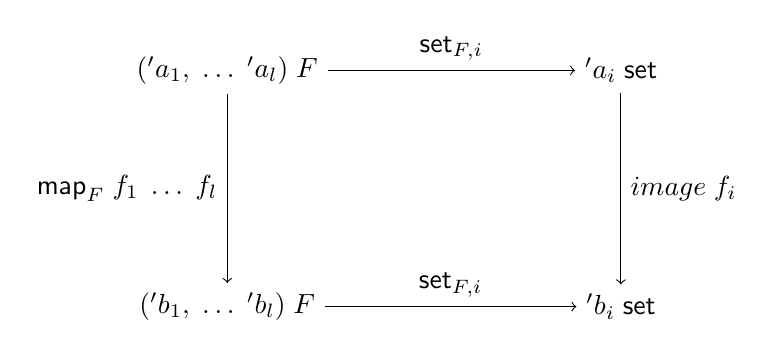
\begin{tikzpicture}[auto]
  % Nodes
  \node (aF) at (0,0) {\(('a_1,\; \dots\; 'a_l)\; F\)};
  \node (bF) at (0,-3) {\(('b_1,\; \dots\; 'b_l)\; F\)};
  \node (aset) at (5,0) {\('a_i\; \textsf{set}\)};
  \node (bset) at (5,-3) {\('b_i\; \textsf{set}\)};

  % Arrows
  \draw[->] (aF) to node[left] {\(\textsf{map}_F\; f_1\; \dots\; f_l\)} (bF);
  \draw[->] (aF) to node {\(\textsf{set}_{F,i}\)} (aset);
  \draw[->] (bF) to node{\(\textsf{set}_{F,i}\)} (bset);
  \draw[->] (aset) to node[right] {\(image\; f_i\)} (bset);
\end{tikzpicture}
\newline
\footnotesize
for all $i$ where $'a_i$ is a live variable of $F$